
% This LaTeX was auto-generated from MATLAB code.
% To make changes, update the MATLAB code and republish this document.

\documentclass{article}
\usepackage{graphicx}
\usepackage{color}

\sloppy
\definecolor{lightgray}{gray}{0.5}
\setlength{\parindent}{0pt}

\begin{document}

    
    
\section*{}


\subsection*{Contents}

\begin{itemize}
\setlength{\itemsep}{-1ex}
   \item LaTeX Markup Example
\end{itemize}


\subsection*{LaTeX Markup Example}

\begin{par}
This is a table:
\end{par} \vspace{1em}
\begin{par}

\begin{tabular}{|c|c|} \hline
$n$ & $n!$ \\ \hline
1 & 1 \\
2 & 2 \\
3 & 6 \\ \hline
\end{tabular}

\end{par} \vspace{1em}
\begin{verbatim}
l = 1
h = 1;
link1  = [ 1 0 0 45];
link2 =  [ 0 90 0 0]
link3 =  [ 16 0 0 0]


links = [link1;link2;link3];
hold on;
set(gca,'YDir','Reverse')
set(gca,'XDir','Reverse')
grid on;
xlabel('X');
ylabel('Y');
zlabel('Z');
A = ones(4,4,length(links(:,1)));
T = ones(4,4,length(links(:,1)));
A = getA(links);
T = getT(A);
x = squeeze(T(1,4,:))
y = squeeze(T(2,4,:));
z = squeeze(T(3,4,:));
x = x';
y = y';
z = z';
xPlot = [0 x];
yPlot = [0 y];
zPlot = [0 z];
plot3(xPlot,yPlot,zPlot,'black','LineWidth',4);
plot3(xPlot(end),yPlot(end),zPlot(end),'x','LineWidth',8);
\end{verbatim}

        \color{lightgray} \begin{verbatim}
l =

     1


link2 =

     0    90     0     0


link3 =

    16     0     0     0


x =

    0.7071
    0.7071
   12.0208

\end{verbatim} \color{black}
    
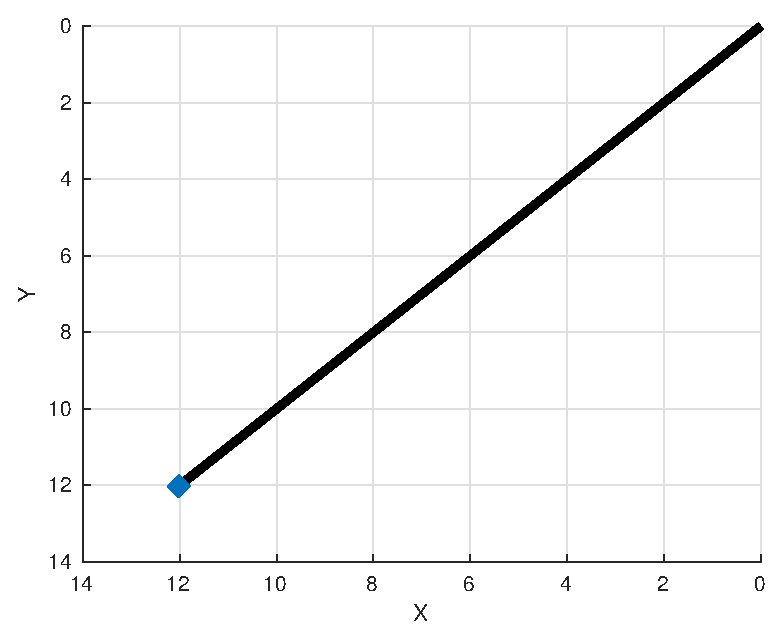
\includegraphics [width=4in]{testArm_01.eps}



\end{document}
    
